\documentclass{standalone}
\usepackage{tikz}

\tikzset{
  svgfrag/.style 2 args={
    execute at begin scope={\special{dvisvgm:raw <g class="fragment #2" data-fragment-index="#1">}},
    execute at end scope={\special{dvisvgm:raw </g>}},
    execute at begin node={\special{dvisvgm:raw <g class="fragment #2" data-fragment-index="#1">}},
    execute at end node={\special{dvisvgm:raw </g>}},
  }
}

\begin{document}
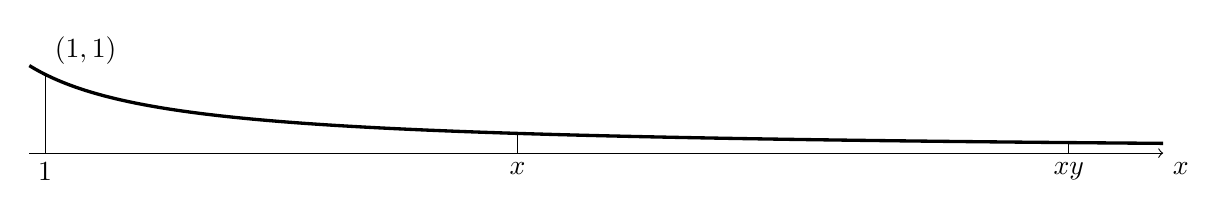
\begin{tikzpicture}[domain=0.9:8.1, yscale=1, xscale=2]
    \draw[->] (0.9,0) -- (8.1,0)node[below right]{$x$};
    \draw[very thick] plot[samples=200] (\x, {1/\x});
    \draw[thin] (1,1)node[above right]{$(1,1)$} -- (1,0)node[below]{$1$};
    \draw[thin] (7.5,0)node[below]{$xy$} -- (7.5,1/7.5);
    \begin{scope}[svgfrag={1}{fade-in}]
        \draw[thin] (4,0)node[below]{$x$} -- (4,1/4);
    \end{scope}
\end{tikzpicture}
\end{document}
